\section{Resultados}\label{sec:resultados}

\subsection{\label{sub:data}Datos}\label{subsec:label{sub:data}datos}

\subsubsection{Primera parte}

Para comprobar el principio de Arqu�medes se toman 3 medidas.

Primero, el sistema cilindro hueco + cilindro macizo en al aire ($P_v$).

Posteriormente, el mismo sistema con el cilindro macizo sumergido en el l�quido ($P_{ap}$).

Por �ltimo, se vierte agua en el cilindro hueco y se toma la medida con el cilindro macizo todav�a sumergido ($P_{ap} + P_{agua}$).

Las tablas~\ref{tab:c-1} y~\ref{tab:c-2} muestran las medidas obtenidas.

\begin{table}[h!]
    \caption{Cilindro macizo 1}
    \label{tab:c-1}
    \begin{centering}
        \begin{tabular}{|P{40px}|P{37px}|P{37px}|P{65px}|}
            \hline
            L�quido   & $P_v\,$(N) & $P_{ap}\,$(N) & $P_{ap} + P_{agua}\,$(N)              \\
            \hline
            \csvreader[late after line= \\, /csv/separator=semicolon ]{./files/data/c-1.csv}{}% use head of csv as column names
            {\csvcoli & \csvcolii  & \csvcoliii    & \csvcoliv}% specify your columns here
            \hline
        \end{tabular}
    \end{centering}
\end{table}

\begin{table}[h!]
    \caption{Cilindro macizo 2}
    \label{tab:c-2}
    \begin{centering}
        \begin{tabular}{|P{40px}|P{37px}|P{37px}|P{65px}|}
            \hline
            L�quido   & $P_v\,$(N) & $P_{ap}\,$(N) & $P_{ap} + P_{agua}\,$(N)              \\
            \hline
            \csvreader[late after line= \\, /csv/separator=semicolon ]{./files/data/c-2.csv}{}% use head of csv as column names
            {\csvcoli & \csvcolii  & \csvcoliii    & \csvcoliv}% specify your columns here
            \hline
        \end{tabular}
    \end{centering}
\end{table}

El principio de Arqu�medes afirma que $P_v$ y $P_{ap} + P_{agua}$ deben ser iguales.

La precisi�n del dinam�metro es $\pm 0.01\,$N, por lo que las medidas obtenidas se encuentran dentro del rango esperado.

\subsubsection{Segunda parte}

\begin{table}[h!]
    \caption{Pesos reales y aparentes en funci�n del n�mero de masas}
    \label{tab:2}
    \begin{centering}
        \begin{tabular}{|P{20px}|P{41px}|P{41px}|P{77px}|}
            \hline
            $n$       & $P_{vac}\,$(N) & $P_{agua}\,$(N) & $(P_{vac} + P_{agua})\,$(N)           \\
            \hline
            \csvreader[late after line= \\, /csv/separator=semicolon ]{./files/data/2_es.csv}{}% use head of csv as column names
            {\csvcoli & \csvcolii      & \csvcoliii      & \csvcoliv}% specify your columns here
            \hline
        \end{tabular}
    \end{centering}
\end{table}



\begin{figure}[h!]
    \begin{center}
        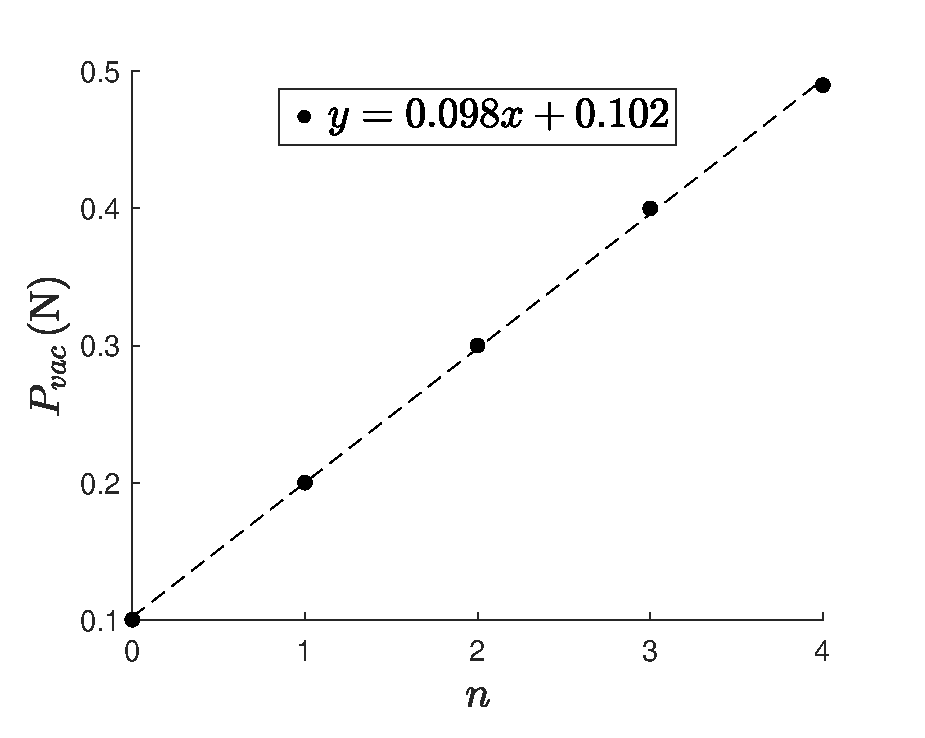
\includegraphics[width=0.8\columnwidth]{files/images/p_vac}
    \end{center}
    \caption{Peso en aire $P_{vac}$ frente al n�mero de pesas}
    \label{fig:p_vac}
\end{figure}

\begin{figure}[h!]
    \begin{center}
        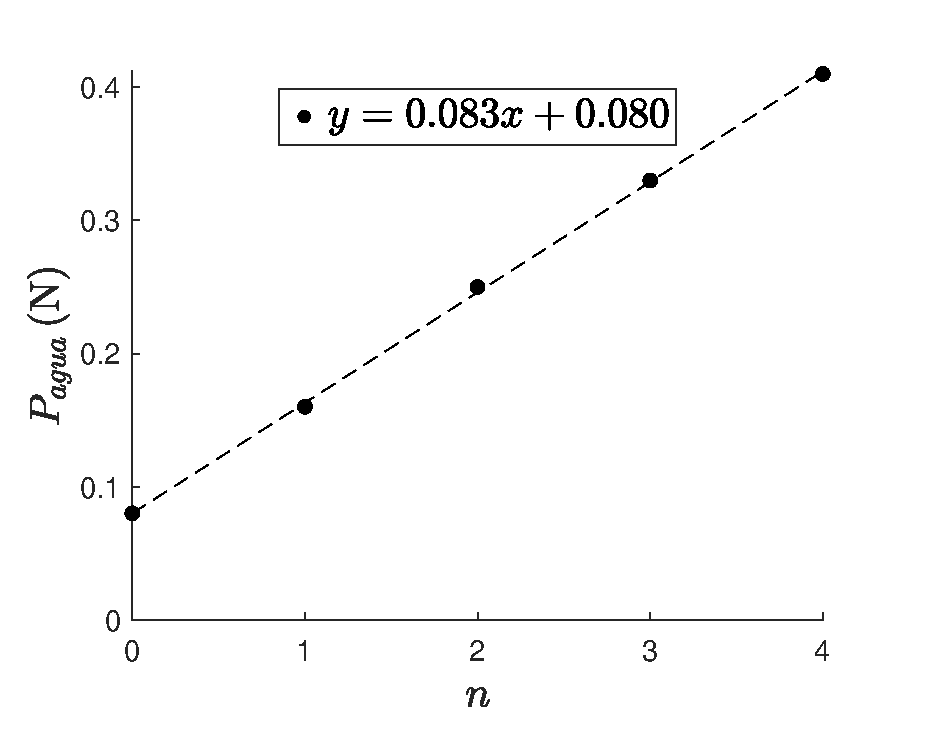
\includegraphics[width=0.8\columnwidth]{files/images/p_agua}
    \end{center}
    \caption{Peso aparente $P_{agua}$ frente al n�mero de pesas}
    \label{fig:p_agua}
\end{figure}

\begin{figure}[h!]
    \begin{center}
        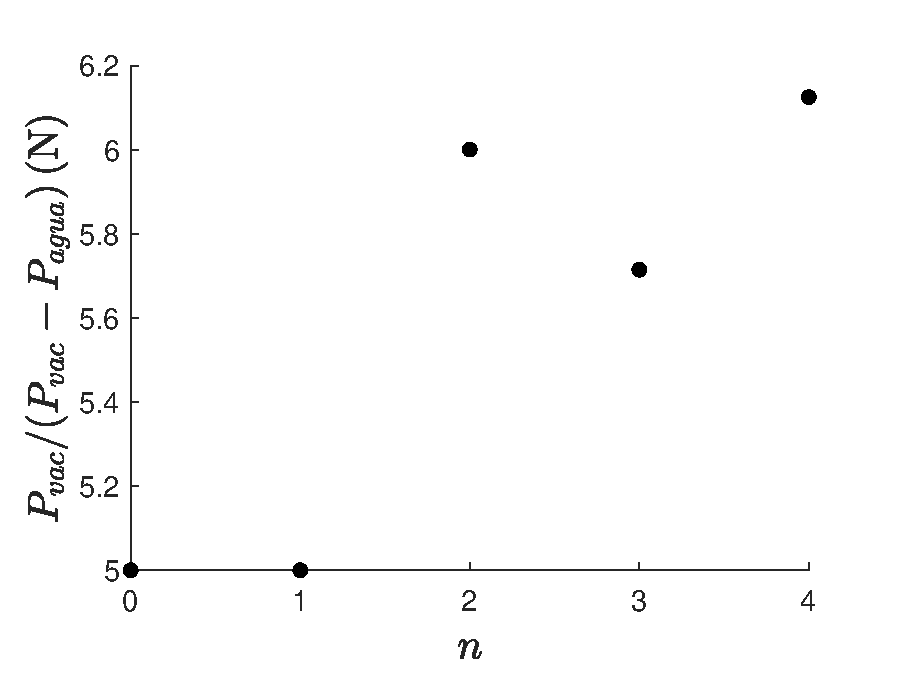
\includegraphics[width=0.8\columnwidth]{files/images/densidad}
    \end{center}
    \caption{$P_{vac}/(P_{vac} - P_{agua})$ frente al n�mero de pesas}
    \label{fig:densidad}
\end{figure}

\subsection{\label{sub:results}An�lisis}\label{subsec:label{sub:results}analisis}

\subsubsection{}

Los valores de la pendiente $a$ y la ordenada en el origen $b$ de la recta de la gr�fica~\ref{fig:p_vac} con sus errores asociados son:
\begin{align*}
    a & = (0.0980 \pm 0.0012)\,\text{(N)}\\
    b & = (0.102 \pm 0.003)\,\text{(N)}\\
\end{align*}

La masa de las pesas es conocida, $m = 10\,$g.

\begin{equation}
    \label{eq:1}
    a = \rho_s \, V_s \, g
\end{equation}

Como $m = \rho_s\, V_s$, despejamos $g$ en la ecuaci�n~\ref{eq:1}:
\begin{equation*}
    g = (9.80 \pm 0.12)\,\text{N/m$^2$}
\end{equation*}

Utilizamos este valor de $g$ para estimar la masa del suspensor.

\begin{equation}
    \label{eq:2}
    b = m_{susp} \, g
\end{equation}

\begin{equation*}
    m_{susp} = (10.41 \pm 0.13)\,\text{g}
\end{equation*}

\subsubsection{\label{subsubsec:densidad_agua}}

\begin{equation*}
    \rho_{s} = \frac{\rho_l}{1 - \frac{a'}{a}}
\end{equation*}

\begin{align*}
    a & = (0.0980 \pm 0.0012)\,\text{(N)}\\
    a' &= (0.0830 \pm 0.0010)\,\text{(N)}\\
\end{align*}


\begin{equation*}
    \epsilon_{\rho_{s}} = \frac{\rho_l}{(1 - \frac{a'}{a})^2} \cdot \frac{1}{a} \cdot \Bigl(\frac{a'}{a}\epsilon_a + \epsilon_a' \Bigr)
\end{equation*}

\begin{align*}
    \rho_s & = (6500 \pm 900)\,\text{kg/m$^3$} \\
    \rho_{susp} &= (4600 \pm 900)\,\text{kg/m$^3$}
\end{align*}

\subsubsection{}

En la figura~\ref{fig:densidad} se observa que la densidad del sistema suspensor pesas parece aumentar con el n�mero de pesas.

Hemos mostrado en la secci�n~\ref{subsubsec:densidad_agua} que el suspensor es de un material m�s ligero que las pesas.

Si sigui�semos a�adiendo pesas, la curva tender�a asint�ticamente a una recta horizontal.

\subsubsection{}

\begin{align*}
    \rho_{vin} & = (6500 \pm 900)\,\text{kg/m$^3$} \\
    \rho_{susp} &= (4600 \pm 900)\,\text{kg/m$^3$}
\end{align*}


